<<<<<<< HEAD
=======
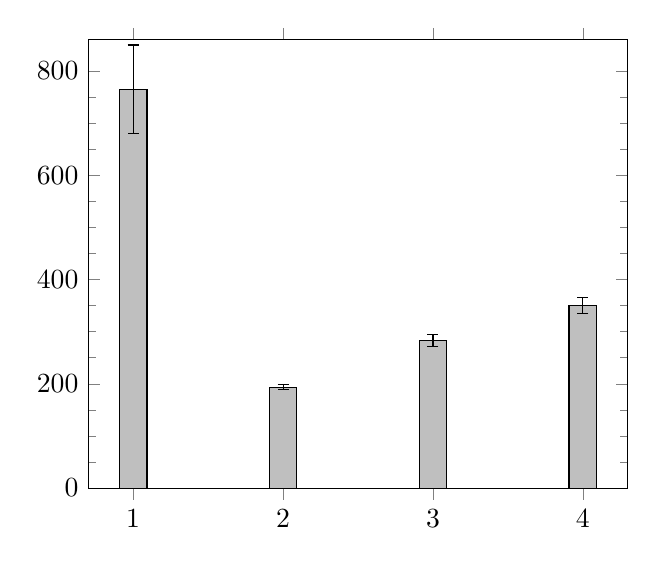
\begin{tikzpicture}

    \begin{axis}[
        xtick = { 1,...,4 },
        xticklabels = { 1, 2, 3, 4 },
        ymax = 860,
        ymin = 0,
        minor y tick num = 3,
        ybar
    ]
    
        \addplot[
            fill = black!25,
            draw = black,
            error bars/.cd,
            y dir = both,
            y explicit
        ]
        table [y error = error] {
            x  y      error  label
            1  765.3  84.7   1
            2  193.3  5.0    2
            3  283.0  11.0   3
            4  350.5  15.9   4
        };
        
    \end{axis}

\end{tikzpicture}
>>>>>>> parent of 88fa715... replace error bars in resistance histogram with second set of data
